\documentclass[12pt]{article}

\usepackage{sbc-template}
\usepackage[brazil,american]{babel}
\usepackage[utf8]{inputenc}

\usepackage{graphicx}
\usepackage{url}
\usepackage{float}
\usepackage{listings}
\usepackage{color}
\usepackage{todonotes}
\usepackage{algorithmic}
\usepackage{algorithm}
\usepackage{hyperref}
\usepackage{indentfirst}
\usepackage{longtable}
\usepackage[inline]{enumitem}


\graphicspath{{./images/}}

\sloppy

\title{Laboratório 5\\- CPU MIPS Pipeline –}

\author{GRUPO 6\\
	Dayanne Fernandes da Cunha, 13/0107191\\
	Lucas Mafra Chagas, 12/0126443\\
	Marcelo Giordano Martins Costa de Oliveira, 12/0037301\\
	Lucas Junior Ribas, 16/0052289\\
	Caio Nunes de Alencar Osório, 16/0115132\\
	Diego Vaz Fernandes, 16/0117925}

\address{Dep. Ciência da Computação -- Universidade de Brasília (UnB)\\
  CiC 116394 - OAC - Turma A
  \email{}
}

\begin{document}
\maketitle

\section{Objetivos}
\label{sec:Objetivos}

\begin{itemize}
\item Treinar o aluno com a linguagem de descrição de \textit{hardware} \textit{Verilog};
\item Familiarizar o aluno com a plataforma de desenvolvimento \textit{FPGA DE2} da \textit{Altera} e o software \textit{QUARTUS II};
\item Desenvolver a capacidade de análise e síntese de sistemas digitais usando uma Linguagem de Descrição de \textit{Hardware};
\item Apresentar ao aluno a implementação de uma \textit{CPU MIPS Pipeline}.
\end{itemize}

\section{Ferramentas}
\label{sec:Materiais}

Todos os códigos escritos neste laboratório podem ser encontrados no repositório \url{https://github.com/Dayof/OAC172} do \textit{GitHub}.

\begin{itemize}
\item FPGA DE2 da Altera 
\item QUARTUS-II
\item Verilog HDL
\end{itemize}

\section{Exercício 2. Análise do processador Pipeline}
\label{sec:pipeline}

\subsection{Diagrama de Blocos do Caminho de Dados}

\begin{figure}[H]
	\flushleft
	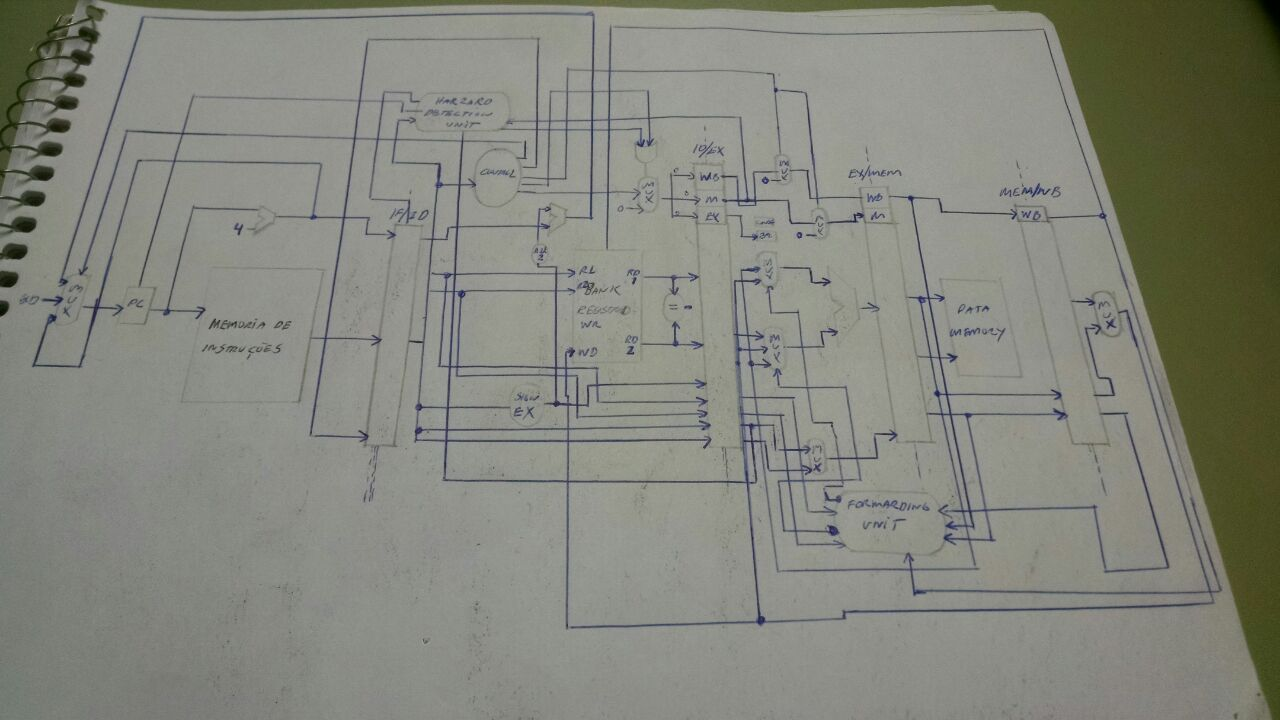
\includegraphics[width=1\textwidth]{pipe.jpg}
	\caption{Caminho de dados - Pipeline.}
	\label{fig:pfunct}
\end{figure}

\subsection{Tabela Verdade dos Sinais de Controle}

\begin{figure}[H]
	\flushleft
	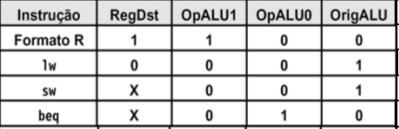
\includegraphics[width=1\textwidth]{ex.png}
	\caption{Controle da execução.}
	\label{fig:pfunct}
\end{figure}
\begin{figure}[H]
	\flushleft
	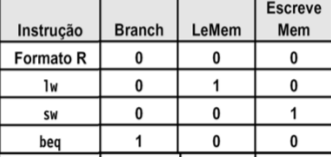
\includegraphics[width=1\textwidth]{mem.png}
	\caption{Controle de acesso a memória.}
	\label{fig:pfunct}
\end{figure}
\begin{figure}[H]
	\flushleft
	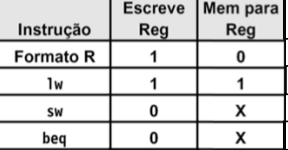
\includegraphics[width=1\textwidth]{escrita.png}
	\caption{Controle de escrita.}
	\label{fig:pfunct}
\end{figure}
\section{Exercício 3. Análise unidades de Hazard e Forward}
\label{sec:hazardforward}

\section{Exercício 4. Teste do funcionamento das instruções da \textit{ISA} }
\label{sec:testeisa}
Foram testadas várias instruções da ISA MIPS atraves do algoritmo teste.s . Alguns exemplos são o ADD, SUB, DIV, MULT, AND, OR...
A demonstração e explicação do código estão presentes nos seguintes vídeos:

\begin{itemize}
\item \href{https://youtu.be/u5eFv9_BDSw}{Formas de Onda}
\item \href{https://youtu.be/PA9af2_Dhi4}{Implementação na DE2} 
\end{itemize}


\section{Exercício 5. Software de lançamento de bola de canhão na \textit{FPGA}}
\label{sec:canhao}

Foi implementado o syscall 6 no algoritmo de simulação do lançamento da bola de canhão. Testes com o teclado foram excutados inserindo velocidades iniciais diferentes de lançamento.

Segue a simulação da bola de canhão:

\href{https://youtu.be/4IZcH5GzhVk}{Bola de canhão}


\section{Exercício 6. Implementação do Cartão SD}
\label{sec:cartaosd}

As limitações observadas ao executar os cenários no cartão sd e impressas no monitor através de um cabo vga foram:

\begin{itemize}
\item A velocidade de acesso a memória do cartão SD é muito lenta comparada a leitura da memória da FPGA, por isso uma boa estratégia é copiar parte dos dados e armazenar na FPGA e após isso efetuar a exibição na tela. Isso sera muito útil no momento dos carregamentos do jogo, aumentando muito a otimzação. 
\end{itemize} 

Segue o vídeo dos cenários:

\href{https://youtu.be/VeoxltP3L6o}{Cenários no cartão SD}

  
\section{Exercício 7. Novas instruções usando a \textit{ISA MIPS}}
\label{sec:isamips} 

\subsection{Parêmtros}
\label{subsec:param}


\subsection{Caminho de dados}
\label{subsec:datapath}


\subsection{Bloco de controle}
\label{subsec:control}


\subsection{Teste das novas instruções}
\label{subsec:testeisa}


\bibliographystyle{sbc}
\bibliography{relatorio}

\end{document}
